% Options for packages loaded elsewhere
\PassOptionsToPackage{unicode}{hyperref}
\PassOptionsToPackage{hyphens}{url}
%
\documentclass[
]{book}
\usepackage{amsmath,amssymb}
\usepackage{lmodern}
\usepackage{iftex}
\ifPDFTeX
  \usepackage[T1]{fontenc}
  \usepackage[utf8]{inputenc}
  \usepackage{textcomp} % provide euro and other symbols
\else % if luatex or xetex
  \usepackage{unicode-math}
  \defaultfontfeatures{Scale=MatchLowercase}
  \defaultfontfeatures[\rmfamily]{Ligatures=TeX,Scale=1}
\fi
% Use upquote if available, for straight quotes in verbatim environments
\IfFileExists{upquote.sty}{\usepackage{upquote}}{}
\IfFileExists{microtype.sty}{% use microtype if available
  \usepackage[]{microtype}
  \UseMicrotypeSet[protrusion]{basicmath} % disable protrusion for tt fonts
}{}
\makeatletter
\@ifundefined{KOMAClassName}{% if non-KOMA class
  \IfFileExists{parskip.sty}{%
    \usepackage{parskip}
  }{% else
    \setlength{\parindent}{0pt}
    \setlength{\parskip}{6pt plus 2pt minus 1pt}}
}{% if KOMA class
  \KOMAoptions{parskip=half}}
\makeatother
\usepackage{xcolor}
\IfFileExists{xurl.sty}{\usepackage{xurl}}{} % add URL line breaks if available
\IfFileExists{bookmark.sty}{\usepackage{bookmark}}{\usepackage{hyperref}}
\hypersetup{
  pdftitle={Excel for General Chemistry},
  pdfauthor={David Hall, David Liu, and Jessica D'eon},
  hidelinks,
  pdfcreator={LaTeX via pandoc}}
\urlstyle{same} % disable monospaced font for URLs
\usepackage{color}
\usepackage{fancyvrb}
\newcommand{\VerbBar}{|}
\newcommand{\VERB}{\Verb[commandchars=\\\{\}]}
\DefineVerbatimEnvironment{Highlighting}{Verbatim}{commandchars=\\\{\}}
% Add ',fontsize=\small' for more characters per line
\usepackage{framed}
\definecolor{shadecolor}{RGB}{248,248,248}
\newenvironment{Shaded}{\begin{snugshade}}{\end{snugshade}}
\newcommand{\AlertTok}[1]{\textcolor[rgb]{0.94,0.16,0.16}{#1}}
\newcommand{\AnnotationTok}[1]{\textcolor[rgb]{0.56,0.35,0.01}{\textbf{\textit{#1}}}}
\newcommand{\AttributeTok}[1]{\textcolor[rgb]{0.77,0.63,0.00}{#1}}
\newcommand{\BaseNTok}[1]{\textcolor[rgb]{0.00,0.00,0.81}{#1}}
\newcommand{\BuiltInTok}[1]{#1}
\newcommand{\CharTok}[1]{\textcolor[rgb]{0.31,0.60,0.02}{#1}}
\newcommand{\CommentTok}[1]{\textcolor[rgb]{0.56,0.35,0.01}{\textit{#1}}}
\newcommand{\CommentVarTok}[1]{\textcolor[rgb]{0.56,0.35,0.01}{\textbf{\textit{#1}}}}
\newcommand{\ConstantTok}[1]{\textcolor[rgb]{0.00,0.00,0.00}{#1}}
\newcommand{\ControlFlowTok}[1]{\textcolor[rgb]{0.13,0.29,0.53}{\textbf{#1}}}
\newcommand{\DataTypeTok}[1]{\textcolor[rgb]{0.13,0.29,0.53}{#1}}
\newcommand{\DecValTok}[1]{\textcolor[rgb]{0.00,0.00,0.81}{#1}}
\newcommand{\DocumentationTok}[1]{\textcolor[rgb]{0.56,0.35,0.01}{\textbf{\textit{#1}}}}
\newcommand{\ErrorTok}[1]{\textcolor[rgb]{0.64,0.00,0.00}{\textbf{#1}}}
\newcommand{\ExtensionTok}[1]{#1}
\newcommand{\FloatTok}[1]{\textcolor[rgb]{0.00,0.00,0.81}{#1}}
\newcommand{\FunctionTok}[1]{\textcolor[rgb]{0.00,0.00,0.00}{#1}}
\newcommand{\ImportTok}[1]{#1}
\newcommand{\InformationTok}[1]{\textcolor[rgb]{0.56,0.35,0.01}{\textbf{\textit{#1}}}}
\newcommand{\KeywordTok}[1]{\textcolor[rgb]{0.13,0.29,0.53}{\textbf{#1}}}
\newcommand{\NormalTok}[1]{#1}
\newcommand{\OperatorTok}[1]{\textcolor[rgb]{0.81,0.36,0.00}{\textbf{#1}}}
\newcommand{\OtherTok}[1]{\textcolor[rgb]{0.56,0.35,0.01}{#1}}
\newcommand{\PreprocessorTok}[1]{\textcolor[rgb]{0.56,0.35,0.01}{\textit{#1}}}
\newcommand{\RegionMarkerTok}[1]{#1}
\newcommand{\SpecialCharTok}[1]{\textcolor[rgb]{0.00,0.00,0.00}{#1}}
\newcommand{\SpecialStringTok}[1]{\textcolor[rgb]{0.31,0.60,0.02}{#1}}
\newcommand{\StringTok}[1]{\textcolor[rgb]{0.31,0.60,0.02}{#1}}
\newcommand{\VariableTok}[1]{\textcolor[rgb]{0.00,0.00,0.00}{#1}}
\newcommand{\VerbatimStringTok}[1]{\textcolor[rgb]{0.31,0.60,0.02}{#1}}
\newcommand{\WarningTok}[1]{\textcolor[rgb]{0.56,0.35,0.01}{\textbf{\textit{#1}}}}
\usepackage{longtable,booktabs,array}
\usepackage{calc} % for calculating minipage widths
% Correct order of tables after \paragraph or \subparagraph
\usepackage{etoolbox}
\makeatletter
\patchcmd\longtable{\par}{\if@noskipsec\mbox{}\fi\par}{}{}
\makeatother
% Allow footnotes in longtable head/foot
\IfFileExists{footnotehyper.sty}{\usepackage{footnotehyper}}{\usepackage{footnote}}
\makesavenoteenv{longtable}
\usepackage{graphicx}
\makeatletter
\def\maxwidth{\ifdim\Gin@nat@width>\linewidth\linewidth\else\Gin@nat@width\fi}
\def\maxheight{\ifdim\Gin@nat@height>\textheight\textheight\else\Gin@nat@height\fi}
\makeatother
% Scale images if necessary, so that they will not overflow the page
% margins by default, and it is still possible to overwrite the defaults
% using explicit options in \includegraphics[width, height, ...]{}
\setkeys{Gin}{width=\maxwidth,height=\maxheight,keepaspectratio}
% Set default figure placement to htbp
\makeatletter
\def\fps@figure{htbp}
\makeatother
\setlength{\emergencystretch}{3em} % prevent overfull lines
\providecommand{\tightlist}{%
  \setlength{\itemsep}{0pt}\setlength{\parskip}{0pt}}
\setcounter{secnumdepth}{5}
\usepackage{booktabs}
\usepackage{amsthm}
\makeatletter
\def\thm@space@setup{%
  \thm@preskip=8pt plus 2pt minus 4pt
  \thm@postskip=\thm@preskip
}
\makeatother
\ifLuaTeX
  \usepackage{selnolig}  % disable illegal ligatures
\fi
\usepackage[]{natbib}
\bibliographystyle{plainnat}

\title{Excel for General Chemistry}
\author{David Hall, David Liu, and Jessica D'eon}
\date{Book last built on 2022-06-08}

\begin{document}
\maketitle

{
\setcounter{tocdepth}{1}
\tableofcontents
}
\hypertarget{preface}{%
\chapter*{Preface}\label{preface}}
\addcontentsline{toc}{chapter}{Preface}

Placeholder

\hypertarget{providing-feedback}{%
\section*{Providing Feedback}\label{providing-feedback}}
\addcontentsline{toc}{section}{Providing Feedback}

\hypertarget{authors}{%
\section*{Authors}\label{authors}}
\addcontentsline{toc}{section}{Authors}

\hypertarget{acknowlegements}{%
\section*{Acknowlegements}\label{acknowlegements}}
\addcontentsline{toc}{section}{Acknowlegements}

\hypertarget{intro}{%
\chapter{Introduction}\label{intro}}

\hypertarget{capabilities}{%
\chapter{Getting Setup for Success}\label{capabilities}}

Placeholder

\hypertarget{accessing-the-microsoft-office-suite-of-software}{%
\section{Accessing the Microsoft Office Suite of Software}\label{accessing-the-microsoft-office-suite-of-software}}

\hypertarget{managing-your-files}{%
\section{Managing your Files}\label{managing-your-files}}

\hypertarget{creating-professional-documents}{%
\section{Creating Professional Documents}\label{creating-professional-documents}}

\hypertarget{adding-an-excel-graph-into-a-word-document}{%
\subsection{Adding an Excel Graph into a Word Document}\label{adding-an-excel-graph-into-a-word-document}}

\hypertarget{creating-a-pdf-from-a-word-document}{%
\subsection{Creating a PDF from a Word Document}\label{creating-a-pdf-from-a-word-document}}

\hypertarget{data-wrangling}{%
\chapter{Data Wrangling}\label{data-wrangling}}

This guide is written for the first-year chemistry courses at the University of Toronto but would be useful for a variety of applications in academia and beyond.

Working in the chemistry lab often involves the production and collection of data. When we collect data in the lab we often feel that any changes, or manipulations, to the data would be dishonest. However, the truth is that most data requires some manipulation as part of its analysis. In this section we will discuss how to import your data into excel (if it's not already in Excel), how to format it and how to make educated, and transparent, decisions related to data manipulation.

\hypertarget{file-upload}{%
\section{File Upload}\label{file-upload}}

Many datasets (particularly larger ones) are stored as .csv files. The CSV file extension stands for comma-separate values file, a popular file format for storing data that you are bound to encounter again in your academic careers. As the name implies, CSV files contain data separated by commas; go ahead and open your file in Notepad/TextEdit or Microsoft Word if you want to see this. Excel can open CSV files and will often automatically assigned the comma-separated values into different columns. Once you open your .csv file using excel be sure to save it as an .xlsx file so that you can avail yourself of all of Excel's features.

gif - saving file with .xlsx extension

\hypertarget{data-organization-and-cell-formatting}{%
\section{Data Organization and Cell Formatting}\label{data-organization-and-cell-formatting}}

When you open your file in Excel you should see data organized into four columns with the following headers:
- Date \& Time: This column indicates the day and time the air quality data was measured.
- Temperature: The ambient air temperature in degrees Celsius.
- NO2: The concentration of NO2 in the air in ppb.
- O3: The concentration of O3 in the air in ppb.

\begin{figure}
\centering
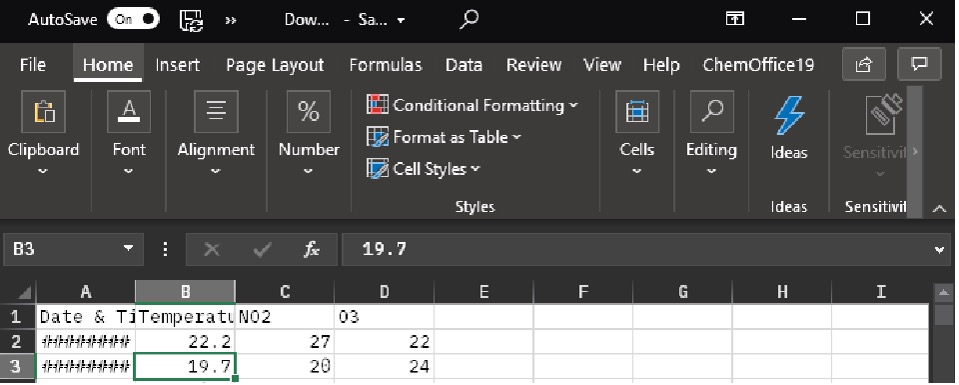
\includegraphics{images/Figure1.jpg}
\caption{\textbf{Figure 1.} Initial layout of Excel and imported data.}
\end{figure}

The temperature and concentration values provided are hour-ending averages, meaning that when you see temperature or concentration for 1 AM, it is the average of the measured values between 12 AM and 1 AM that day.

Notice how the values are arrayed in a table of cells, each containing a single value. These cells are arranged in columns with labelled headings (A, B, C, etc.) and rows (1, 2, 3, etc.). A single cell can be referenced using this system (i.e.~in the image above the cell ``B3'' contains the value 19.7).

Excel displays pound signs (\#\#\#) if a cell is too narrow to display the value. You can manually adjust the width of columns by dragging the boundary on the right side of the column heading or double clicking the right boundary to automatically adjust it to the width of its contents.

gif - how to resize the column - also need to remake the figure above to match the gif

If any of your cells are not properly formatted, right click on them and select \emph{Format Cells\ldots{}} from the dropdown menu (you can also go to the \emph{Format} menu and select \emph{Cells\ldots{}}). In the \emph{Format Cells} dialog box (Figure 2) you can see many formatting options, some of which are described in Table 1. If your dataset includes a date you can format it so that it shows both the date and the time using the \emph{Custom} category and the yyyy-mm-dd h:mm formatting option as shown in Figure 3.

\begin{figure}
\centering
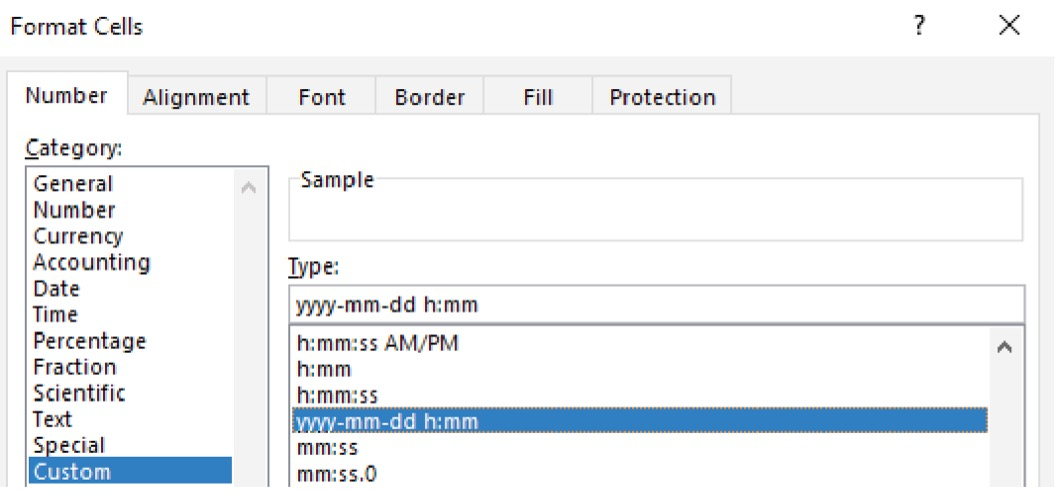
\includegraphics{images/Figure3.jpg}
\caption{\textbf{Figure 2.} The FORMAL CELLS dialog box.}
\end{figure}

Some useful number formats are provided in Table 1. If your data includes a date and time component it is important to note that Excel stores date values as the number of days since 1900-Jan-0, with a decimal value corresponding to the time of day. In the example in Table 1, 44005 days have passed since then, so Excel can interpret this as a date value. This also goes the other way when your numerical value may incorrectly be interpreted as a date. Just remember that the formatting only affects how the numbers are displayed, not the numbers themselves.

\begin{longtable}[]{@{}llr@{}}
\toprule
Category & Description & Example \\
\midrule
\endhead
General & Has no sp & ecific format and so for numbers returns the full numerical value 44005 \\
Number & General d & isplay of numbers, can adjust the number of decimal places 44005.00 \\
Scientific & & \\
Date (long) & & \\
Date (short) & & \\
Custom & & \\
\bottomrule
\end{longtable}

\begin{longtable}[]{@{}
  >{\raggedright\arraybackslash}p{(\columnwidth - 4\tabcolsep) * \real{0.3333}}
  >{\raggedright\arraybackslash}p{(\columnwidth - 4\tabcolsep) * \real{0.3333}}
  >{\raggedright\arraybackslash}p{(\columnwidth - 4\tabcolsep) * \real{0.3333}}@{}}
\toprule
\begin{minipage}[b]{\linewidth}\raggedright
Category
\end{minipage} & \begin{minipage}[b]{\linewidth}\raggedright
Description
\end{minipage} & \begin{minipage}[b]{\linewidth}\raggedright
Example
\end{minipage} \\
\midrule
\endhead
General & Has no specific format and so for numbers returns the full numerical value & 44005 \\
Paragraph & Text & \\
\bottomrule
\end{longtable}

\hypertarget{data-manipulation}{%
\section{Data Manipulation}\label{data-manipulation}}

The word \emph{manipulation} has a sinister connotation when referring to people, but in reference to data it is anything but. Data manipulation is the process of creating useful and meaningful datasets from which useful and meaningful information can be obtained. An example \emph{what} and \emph{why} of data manipulation can be found in the NAPS air quality datasets.

If you create a timeseries for your NAPS data (details on instructions for this) you may see something similar to the plot shown below. Does anything stand out about this plot? Are there any outliers or points that differ significantly from the others?

Figure with -999 value

In this timeseries there is one point that is immediately suspicious. Our y-axis represents the concentration of either O3 or NO2, and one point has a reported concentration value of around -- 1000 ppb, a physical impossibility. This issue arises because the value of -999 denotes no data was available because there was an issue with the instrument. Maybe the instrument didn't collect data, or it reported a failed calibration, or any number of other possible issues. In designing the data collection system a value of -999 was used when this happens so it is immediately noticeable, unlike a missing value which could be misinterpreted as zero.

It is clear this value of -999 will need to be removed, but how? Do we need to go through all 168 concentration values to find this outlier? Of course not! This is where we start to explore functions and operations in spreadsheet software to do this work for us! Below is a description of the \emph{Find and Replace} function in Excel that can be used to remove these -999 values.

There are many many other data manipulation strategies and techniques which you will use throughout your time in the first year chemistry labs and beyond

How to end this section? Maybe with a comment on how visuzling the data was a useful way to assess the data?

\hypertarget{find-and-replace-function}{%
\subsection{Find and Replace Function}\label{find-and-replace-function}}

The find and replace function is useful if you need to find data in your Excel sheet. For the NAPS data, if you have -999 values in your dataset you will need to find and remove it before proceeding as it will interfere with your analysis and visualization. If you're not sure whether you have a -999 value in your dataset this is also a great way to look and see! One way to approach this issue is to enter `-999' in the search bar at the top right of the screen and then delete any of these values manually leaving a blank cell behind.

gif - using the search bar to look for -999 values

Alternatively, if you would like to get Excel to do this work for you, you can select \emph{Edit} on the top menu, then select \emph{Find} and then \emph{Replace\ldots{}}. In the \emph{Find and Replace} dialog box input -999 into the \emph{Find What:} box and leave the \emph{Replace with:} box empty. Then click \emph{Replace All} and Excel will replace all the -999 values with blank cells and tell you how many instances the -999 value was replaced. If you have a plot already created from this data it should be updated automatically.

gif - using the find and replace function

Replacing the -999 values with blanks will not work if you need to use those values in a calculation, as Excel will assume the missing values are zeros, which is not true. To fix this issue you will need to remove any rows with missing data. To do this, highlight all the columns involved (A-E in this example), select the \emph{Edit} menu, then \emph{Find}, and \emph{Go To}. In the \emph{Go To} dialog box click on \emph{Special}. In the \emph{Go To Special} dialog box select \emph{Blanks}, then click \emph{OK}. This will highlight any cells that are blank in the columns you highlighted.

gif - selecting all the columns

You can remove the rows manually by right clicking on the row number and selecting \emph{Delete} from the dropdown menu. Alternatively, with the blank cells highlighted, you can select the \emph{Home} ribbon, then click on the arrow next to the \emph{Delete} button, then select \emph{Delete Sheet Rows} in the dropdown menu. Both approaches lead to the same outcome. No matter the approach it is important to delete the entire row, otherwise Excel will move the values up in that column only, which will alter the dataset. Once you remove all the relevant rows scroll to the bottom of your dataset and ensure the columns are of equal length, if not, you may have accidentally deleted a single cell rather than the entire row.

gif - deleting rows the two ways and then checking that the data table is still the same length

\hypertarget{mathematical-operations-and-simple-statistics}{%
\chapter{Mathematical Operations and Simple Statistics}\label{mathematical-operations-and-simple-statistics}}

Many aspects of chemistry are quantitative, meaning we use mathematical operations to explain and explore chemical phenomena. This math can be done by hand, but once you have more than one or two data points this gets very tiring and a spreadsheet can be a lifesaver! In this section we will talk about how to program mathematical equations into excel, how to use common mathematical functions, and how to reference other values within the spreadsheet. We will also dip our toes into some simple programming language that can be very helpful.

\hypertarget{mathematical-operations}{%
\section{Mathematical Operations}\label{mathematical-operations}}

Excel can perform many mathematical operations and Table 2 shows a number of the common operations with the corresponding formula.

Table 2

Recall chemical equations {[}1{]} to {[}3{]} from the introduction that describe the relationship between NO2 and O3.

how to add equations?

\[E = mc^2\]

Also, recall that because these two pollutants are so intimately linked atmospheric chemists have defined a term called ``odd oxygen'' or OX that is the sum of NO\textsubscript{2} and O\textsubscript{3} at a given time point.

To add OX to your analysis first calculate the concentration OX at each timepoint in your dataset. Details on how to perform simple mathematical operations in Excel can be found in {[}website link{]}.

\hypertarget{data-visualization}{%
\chapter{Data Visualization}\label{data-visualization}}

This is an R Markdown document. Markdown is a simple formatting syntax for authoring HTML, PDF, and MS Word documents. For more details on using R Markdown see \url{http://rmarkdown.rstudio.com}.

When you click the \textbf{Knit} button a document will be generated that includes both content as well as the output of any embedded R code chunks within the document. You can embed an R code chunk like this:

\begin{Shaded}
\begin{Highlighting}[]
\FunctionTok{summary}\NormalTok{(cars)}
\end{Highlighting}
\end{Shaded}

\begin{verbatim}
##      speed           dist       
##  Min.   : 4.0   Min.   :  2.00  
##  1st Qu.:12.0   1st Qu.: 26.00  
##  Median :15.0   Median : 36.00  
##  Mean   :15.4   Mean   : 42.98  
##  3rd Qu.:19.0   3rd Qu.: 56.00  
##  Max.   :25.0   Max.   :120.00
\end{verbatim}

\hypertarget{including-plots}{%
\section{Including Plots}\label{including-plots}}

You can also embed plots, for example:

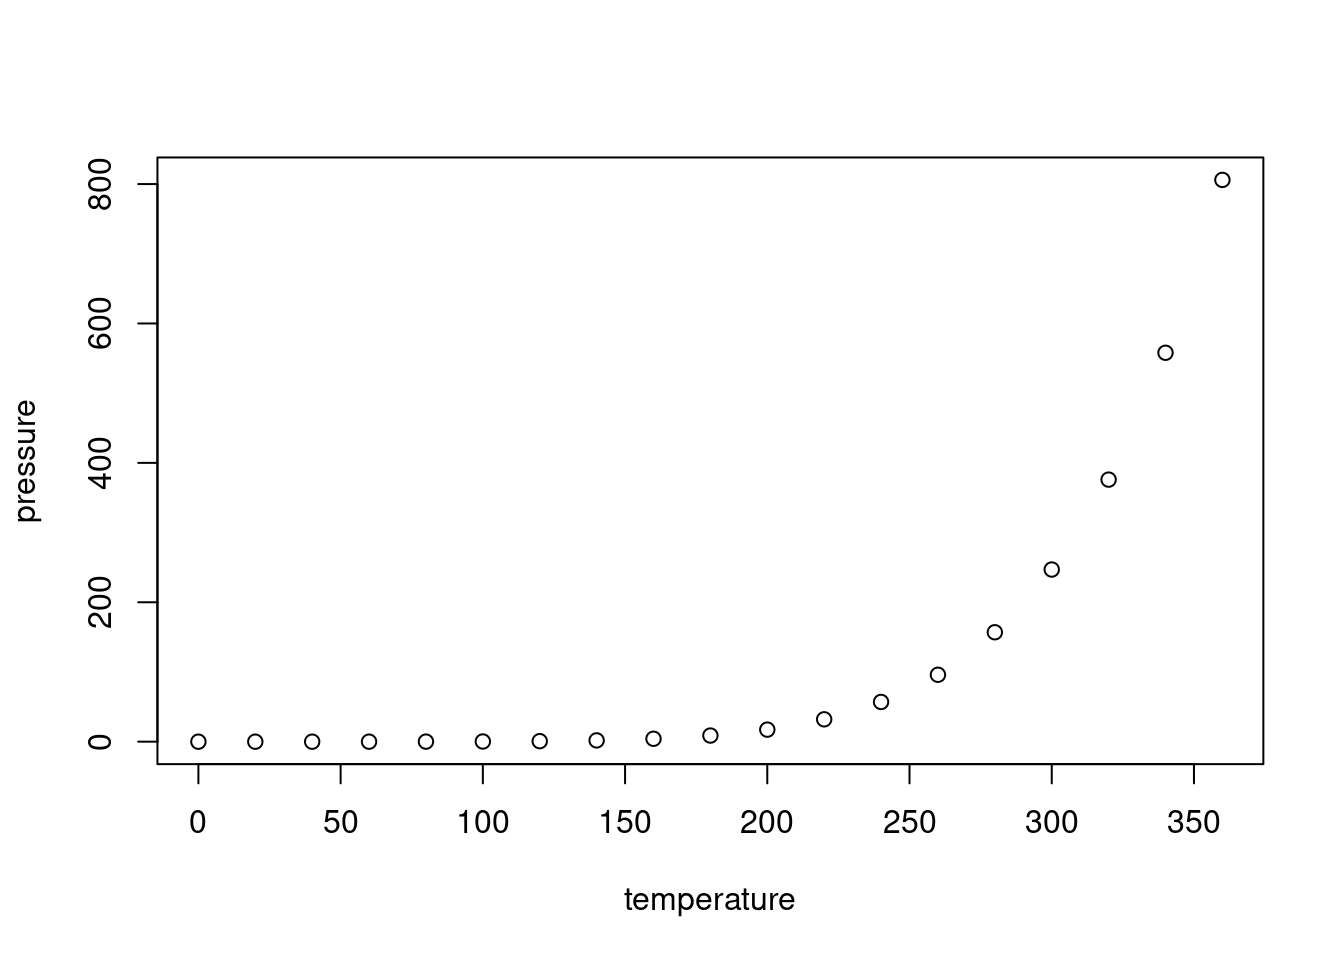
\includegraphics{excel4chem_files/figure-latex/pressure-1.pdf}

Note that the \texttt{echo\ =\ FALSE} parameter was added to the code chunk to prevent printing of the R code that generated the plot.

\hypertarget{bookdown-capabilities}{%
\chapter{Bookdown Capabilities}\label{bookdown-capabilities}}

Placeholder

\hypertarget{interactive-and-exportable-tables}{%
\section{Interactive and exportable tables}\label{interactive-and-exportable-tables}}

\hypertarget{animated-gifs}{%
\section{Animated GIFS}\label{animated-gifs}}

\hypertarget{embedded-videos}{%
\section{Embedded videos}\label{embedded-videos}}

\hypertarget{jessica-test-woo-hoo}{%
\section{Jessica Test, Woo hoo!}\label{jessica-test-woo-hoo}}

  \bibliography{book.bib,packages.bib}

\end{document}
